\documentclass{article}
\usepackage[margin=1.125in]{geometry}
\usepackage{graphicx}
\usepackage{float}
\begin{document}
\section{Introduction} 
%Paragraph 1
%A major challenge in theoretical physics is the development of an accurate effective low-energy theory for the cuprate superconductors. The cuprate materials all share a common feature of repeating charge reservoir layers and CuO$_2$ planes within the conventional unit cell, with the reservoir layers providing hole or electron carriers to the CuO$_2$ planes under doping. The parent material to the cuprates are charge-transfer insulators with anti-ferromagnetic (AFM) order [ref]. The common phases shared by all cuprate materials are the AFM, pseudogap, strange metallic, normal metallic, and superconducting phases, with each phase deviating from the simple behavior we expect from  The pseudogap phase exists in the underdoped region with T$>$T$_c$ but still maintains a gap [ref]. The strange metal phase appears in the optimally doped region above T$_c$ and is a metallic phase, but has linear resistivity as opposed to the quadratic resisitivity expected from a Fermi-Landau liquid theory [ref]. The normal metal phase has Fermi-Landau like single-particle charge excitations (quasiparticle excitations), but does not have the predicted bosonic charge excitations (plasmons) [ref]. The superconducting phase has d$_{x^2-y^2}$ pairing and lives under a superconducting dome with the transition temperature T$_c$ varying with doping. 
%

%Paragraph 2
%The difficulty can be attributed in large part to the host of structural, magnetic and charge orders that exist as doping, temperature and pressure are varied. The simplest orders that are shared among all cuprates are charge transfer anti-ferromagnetic, pseudogap, strange metallic, normal metallic, and superconducting phases which stabilize as doping and temperature are varied \textbf{[ref1]}. Alongside these common orders, particular cuprate families exhibit structural phase transitions\textbf{[ref2]}, static stripe-like order\textbf{[ref3, ref4, ref5]}, and charge density wave order \textbf{[ref6]}. 
%

%Paragraph 3
%Paragraph 5

%Paragraph 4 + 6 merge 
%We propose that a density matrix downfolding approach using \textit{ab initio} Quantum Monte Carlo calculations can generate an effective model which can accurately describe low-energy properties and energetics for t%he infinite layer electron-doped cuprates at T=0 and x=0, 0.125, 0.25. 

\section{Preliminary results}
In order to become acquainted with our code QWalk [ref QWalk] and QMC algorithms in general I worked on implementing and testing multi-Slater-Jastrow trial functions with optimized non-orthogonal determinants (MSJ+NO) in FN-DMC [ref my paper]. We assessed the efficiency and compactness of this new trial function by calculating the ground state energy and single particle densities of a C$_2$ molecule using FN-DMC and comparing to the results when using multi-Slater-Jastrow trial functions with optimized orthogonal determinant trial functions (MSJ+O). The workflow involved constructing the un-optimized trial wave functions, optimizing the parameters using an energy optimization method [ref], and finally using the optimized trial functions in an FN-DMC calculation. We found that the FN-DMC energy calculated using an MSJ+NO trial function with only 24 determinants was lower than the FN-DMC energy using an MSJ+O trial function with 55 determinants. Further, the FN-DMC charge density calculated using MSJ+NO trial functions had stronger bonding character than when using MSJ+O trial functions, a reasonable result as introducing correlations into trial functions allows for electrons to avoid each other while still occupying the same bonding region. Our results indicated that using non-orthogonal determinants may lead to more compact multi-Slater-Jastrow trial wave functions for small molecules.

Before moving on to the computationally expensive DMD with FN-DMC calculations on SrCuO$_2$, we attempted an \textit{ad hoc} model fitting procedure using only eigenvalues and total energies from density functional theory (DFT) to get a grasp on the relevant energy scales, model terms, and values for model parameters. A single DFT calculation provides us three pieces of information: a Slater determinant wave function with occupied single particle orbitals $|\Psi_{DFT}\rangle$, a single particle band structure which represents the DFT eigenvalues $\epsilon(\vec{k})_{DFT}$, and a total DFT energy $E_{DFT}$. Suppose we have some low-energy effective model in mind with parameters $\vec{p}$, H$_m$($\vec{p}$). We can fit the parameters in the model using only information from the DFT calculation by constructing a cost function which depends on $\vec{p}$, and then minimizing the cost. The cost function we used was:
\begin{equation}
Cost(w_E, \vec{p}) = \sum_{i=1}^{n} [\sum_{\vec{k}}(\epsilon(\vec{k})_{DFT,i} - \epsilon(\vec{k})_{m,i})^2] + w_E[E_{DFT,i} - \langle \Psi_{DFT,i}|H_m(\vec{p})| \Psi_{DFT,i} \rangle]^2
\end{equation}
where the sum over $i$ is over a sample of low-energy DFT states. The first term is the cost function for a least squares fit of the single particle eigenvalues calculated using our model $\epsilon(\vec{k})_m$ and the DFT state $|\Psi_{DFT,i}\rangle$ to the DFT eigenvalues. The second term is a cost function for a least squares fit of the total energy calculated using our model to the DFT total energy. The term $w_E$ controls the importance of minimizing the total energy cost relative to the eigenvalue cost, and is a variable parameter. The accuracy of the fit was assessed by looking at the $R^2$ value between the total energies, $R^2_E$, and between the eigenvalues, $R^2_\epsilon$. The fitting procedure then follows: choose a model Hamiltonian H$_m$, choose a sequence of $w_E$, minimize the cost function for each $w_E$ in the sequence and obtain a sequence of tuples $(\vec{p}, R^2_E, R^2_\epsilon)$. Increasing $R^2_E$ to near 1.0 will lead to a decrease in $R^2_\epsilon$ and vice versa, so the optimal model parameters are chosen by conducting a Pareto efficiency analysis on the sequence of pairs $(R^2_E, R^2_\epsilon)$. The Pareto optimal pair then gives us the optimal parameters $\vec{p}^\star$. Note that the resulting fitted effective model will not accurately reproduce the low-energy features of the \textit{ab initio} Hamiltonian H, but rather will reproduce the low-energy features of the effective Kohn-Sham theory used in our DFT calculation.

We conducted this \textit{ad hoc} fitting procedure for SrCuO$_2$ under three different dopings x=0, 0.125, and 0.25 using the PBE0 functional in DFT on a 2$\sqrt{2}$x2$\sqrt{2}$x1 unit cell. The PBE0 functional has been used within QMC in the past to yield accurate results for low-energy properties and energies on the hole-doped cuprates [ref]. The eight unit cell calculation was chosen since it is small enough to be computationally feasible even when moving to QMC, but large enough that the finite size effects are not too large. For the undoped calculations, the PBE0 ground state was a checkerboard AFM state, and the six low-energy states we considered were states with spins flipped relative to this ground state. This choice was made since the lowest energy excitations of the undoped cuprates are spin excitations as they are charge-transfer insulators. For the x=0.125 calculations, the PBE0 ground state was a flip state, and the four low-energy states we considered were states with total energy less than 0.25 eV above this ground state. One excited state in this energy range was discarded because it was insulating in character while the other four were metallic. This may have occured since PBE0 has been shown to incorrectly order states energetically for strongly correlated systems [ref]. For the x=0.25 calculations, the PBE0 ground state was a collinear state, and the four low-energy states we chose were states with total energy less than 0.30 eV above this ground state. Again one state in this range was insulating, while the other four were metallic, and this state was discarded from the fitting procedure. The model we chose to fit has four terms: 
\begin{equation}
H_m = -t \sum_{\langle i,j \rangle} c_i^\dagger c_j + h.c.
+ t^\prime\sum_{\langle \langle i.j \rangle \rangle} c_i^\dagger c_j + h.c. +\\
K\sum_{\langle i,j \rangle} \vec{S_i} \cdot c_{j,\alpha}^\dagger \vec{\sigma}_{\alpha,\beta} c_{i,\beta} + J \sum_{\langle i,j \rangle} \vec{S_i} \cdot \vec{S_j}.
\end{equation}
The operators $\vec{S_i}$ represent the spin moment on the copper sites and $c_i^\dagger$ the itinerant electrons hopping around copper sites. The last term is a Heisenberg exchange which we included since the undoped material can be modeled fairly accurately with just a nearest neighbor Heisenberg model with J = 0.18 eV [ref]. The first two terms are nearest neighbor and next-nearest neighbor hopping which are both required to capture the curvature of the PBE0 bands crossing the Fermi level for the x=0.125 and x=0.25 low-energy states. The third term is a nearest neighbor Kondo term which we included since it can help stabilize a flip state over a checkerboard state, as seen in the x=0.125 PBE0 calculations. In order to extract the band structure and total energy from this model we made a mean field approximation where we split the electrons into two groups: those which contribute to the fixed spin moments $\vec{S_i}$ on site and those which are itinerant $c_i^\dagger$. This choice was motivated by looking at the PBE0 band structures of the low-energy states. As shown in \ref{fig3} the band structure is split by a large gap on the order of 1 eV, in this case for the collinear x=0.25 state. The bands above this gap cross the Fermi level, and can be thought of as bands which contribute only itinerant electrons. The bands below this gap never cross the Fermi level, and can be thought of as bands which contribute only to the fixed spin moments on copper sites. Therefore we can treat the quantities $\vec{S_i}$ as fixed variables, the values of which are dictated by the bands below the gap for a given PBE0 calculation. In doing so, the Kondo term becomes a 1-body term and the Heinsenberg term becomes a constant value, leaving the model Hamiltonian as a 1-body Hamiltonian which we can exactly diagonalize to get the total energy and eigenvalues. 

We find that the four term model above can accurately describe the PBE0 band structures and total energies of low-energy states of SrCuO$_2$ for x=0, 0.125, and 0.25. \ref{fig4} shows the results of our \textit{ad hoc} fitting procedure. For the undoped calculation no fitting to eigenvalues was necessary nor Pareto efficiency analysis since there were no itinerant electrons, leading to an optimal fit of $t=t^\prime=K=0 eV; J = 0.18 eV$. For the doped calculations, we held J fixed at the undoped value. This choice was made since doping with just one or two electrons in the unit cell means that most nearest neighbor copper atoms will not see the presence of the itinerant electron permanently, meaning that the local exchange interaction will not be too strongly affected. Computationally, holding the value of J fixed at some prior made the minimization of the cost function much more stable. For the doped calculations, the first inset figure shows the Pareto plot with the sequence of $(R^2_E, R^2_\epsilon)$, and the Pareto optimal pair as a blue square. The other five insets show the fits to the bands and total energies from DFT using our model with the Pareto optimal parameters. For the x=0.125 calculation the optimal parameters were with $t,t^\prime,K,J$=1.15, 0.39, -0.29, 0.18 eV $R^2_E$=0.98 and $R^2_\epsilon$=0.96. For the x=0.25 calculation the optimal parameters were $t,t^\prime,K,J$=1.04, 0.53, -0.15, 0.18 eV with $R^2_E$=0.91 and $R^2_\epsilon$=0.94. In both our model and PBE0, the bands which cross the Fermi level are antibonding Cu 3d$_{x^2-y^2}$ orbitals which have been relaxed via small contributions from nearest neighbor oxygen p orbitals. In PBE0 the net spin moments comprised of the bands below the Fermi level also reside on the Cu 3d$_{x^2-y^2}$ orbital, indicating that unlike the hole-doped cuprates where oxygen and copper orbitals both play an important role in the effective theories, the electron-doped cuprates may be simpler since the major players is just the Cu 3d$_{x^2-y^2}$ orbital. Therefore the fact that $t, t^\prime$ have the same sign makes sense as this is a feature arising from the symmetry of the 3d$_{x^2-y^2}$ orbital. The positive sign of $J$ indicates a preference of nearest neighbor spin moments to be anti-ferromagnetically aligned, whereas the negative sign of $K$ shows a preference for itinerant electrons to ferromagnetically align with nearby spin moments. The opposite signs of J and K, and the fact that K is larger in magnitude than J when x=0.125 can lead to the stabilization of a flip state instead of a checkerboard one in PBE0. 

Our first step into DMD with FN-DMC was the generation of appropriate basis elements for our effective model Hamiltonian which we handled for all three dopings using intrinsic atomic orbitals. The \textit{ad hoc} fitting procedure we conducted provided us with a starting point for generating low-energy states for the DMD calculation, the terms in our model Hamiltonian, and parameter values, but gave us no headway on understanding which basis elements to use. Using MOs in our model is not feasible because the interactions we are looking at are local and are nearest neighbor spatially. If our interaction terms were more easily written in a momentum representation then MOs from PBE0 would be a useful basis to use. We could start with atomic orbitals, AOs, which are the building blocks of the MOs in our PBE0 calculation, but AOs in general are not orthogonal to each other. This complicates our model representation because we typically work with models where creation and annihilation operators generate orthogonal states. Therefore, what we are looking for are orbitals that are maximally localized and still orthogonal to one another, and this is precisely what the IAO is [ref]. In order to test whether the IAO basis is sufficient at spanning the space of excitations we are interested in, we looked at the 1-body reduced density matrix (1RDM) relative to the IAO basis for each x=0, 0.125 and 0.25 low-energy state chosen above. We found that the total number of electrons in the system is accounted for up to three decimal places using just the trace of the 1RDM over the minimal IAO basis. Further, we found that the primary variation between low energy states at a fixed doping was in occupation of the IAOs was of the 3$d_{x^2-y^2}$ IAO. For the undoped calculations the only variation in IAO occupation among the various states was the relative occupation of the spin-up or spin-down 3$d_{x^2-y^2}$ orbital on particular copper sites. This makes sense as the only difference between the undoped low-energy states was the configuration of local spin moments. Under doping, the primary variation in orbital occupation was found in the 3$d_{x^2-y^2}$ IAO which had the lower occupancy. This makes sense as the only place the added electron can go is in the 3$d_{x^2-y^2}$ orbital in the spin channel opposite to the local moment on the site. \ref{fig5} shows the IAOs for the majority spin IAO, which has the higher occupation, and the minority spin IAO, which has the lower spin, for a low-energy state at x=0.125. It is clear that the majority spin IAO is more tightly localized on site whereas the minority spin IAO spreads across the unit cell with contributions from oxygen p-orbitals. We therefore come to the conclusion that the majority spin IAOs should be used as a basis for the localized spin moments, $\vec{S_i}$, and the minority spin IAOs should be used as a basis for the itinerant electrons, $c_i^\dagger$. 

\begin{figure}[H]
\centering
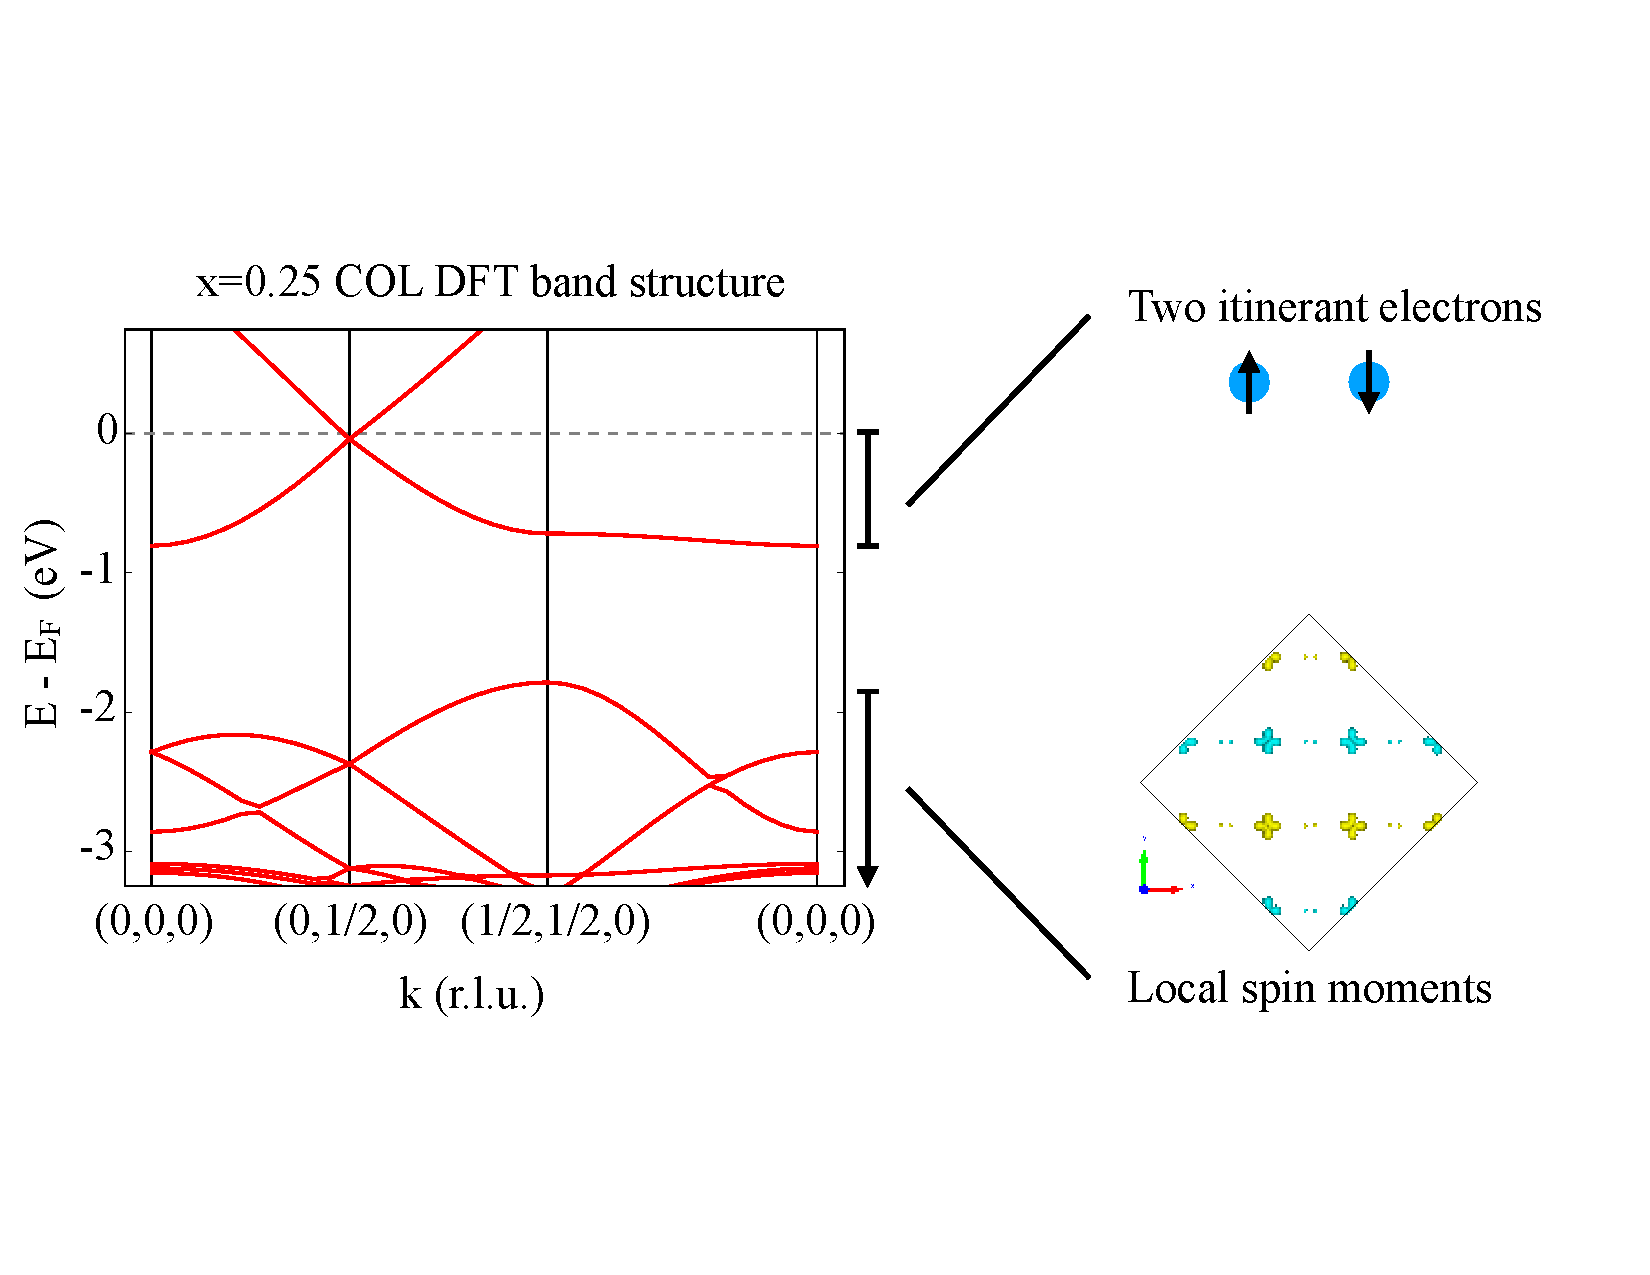
\includegraphics[width=0.6\textwidth]{Figures/R1-mean_field.pdf}
\caption{\label{fig3} Schematic diagram showing the method for mean-field approximation we used in our DFT model fitting calculations.}
\end{figure}

\begin{figure}[H]
\centering
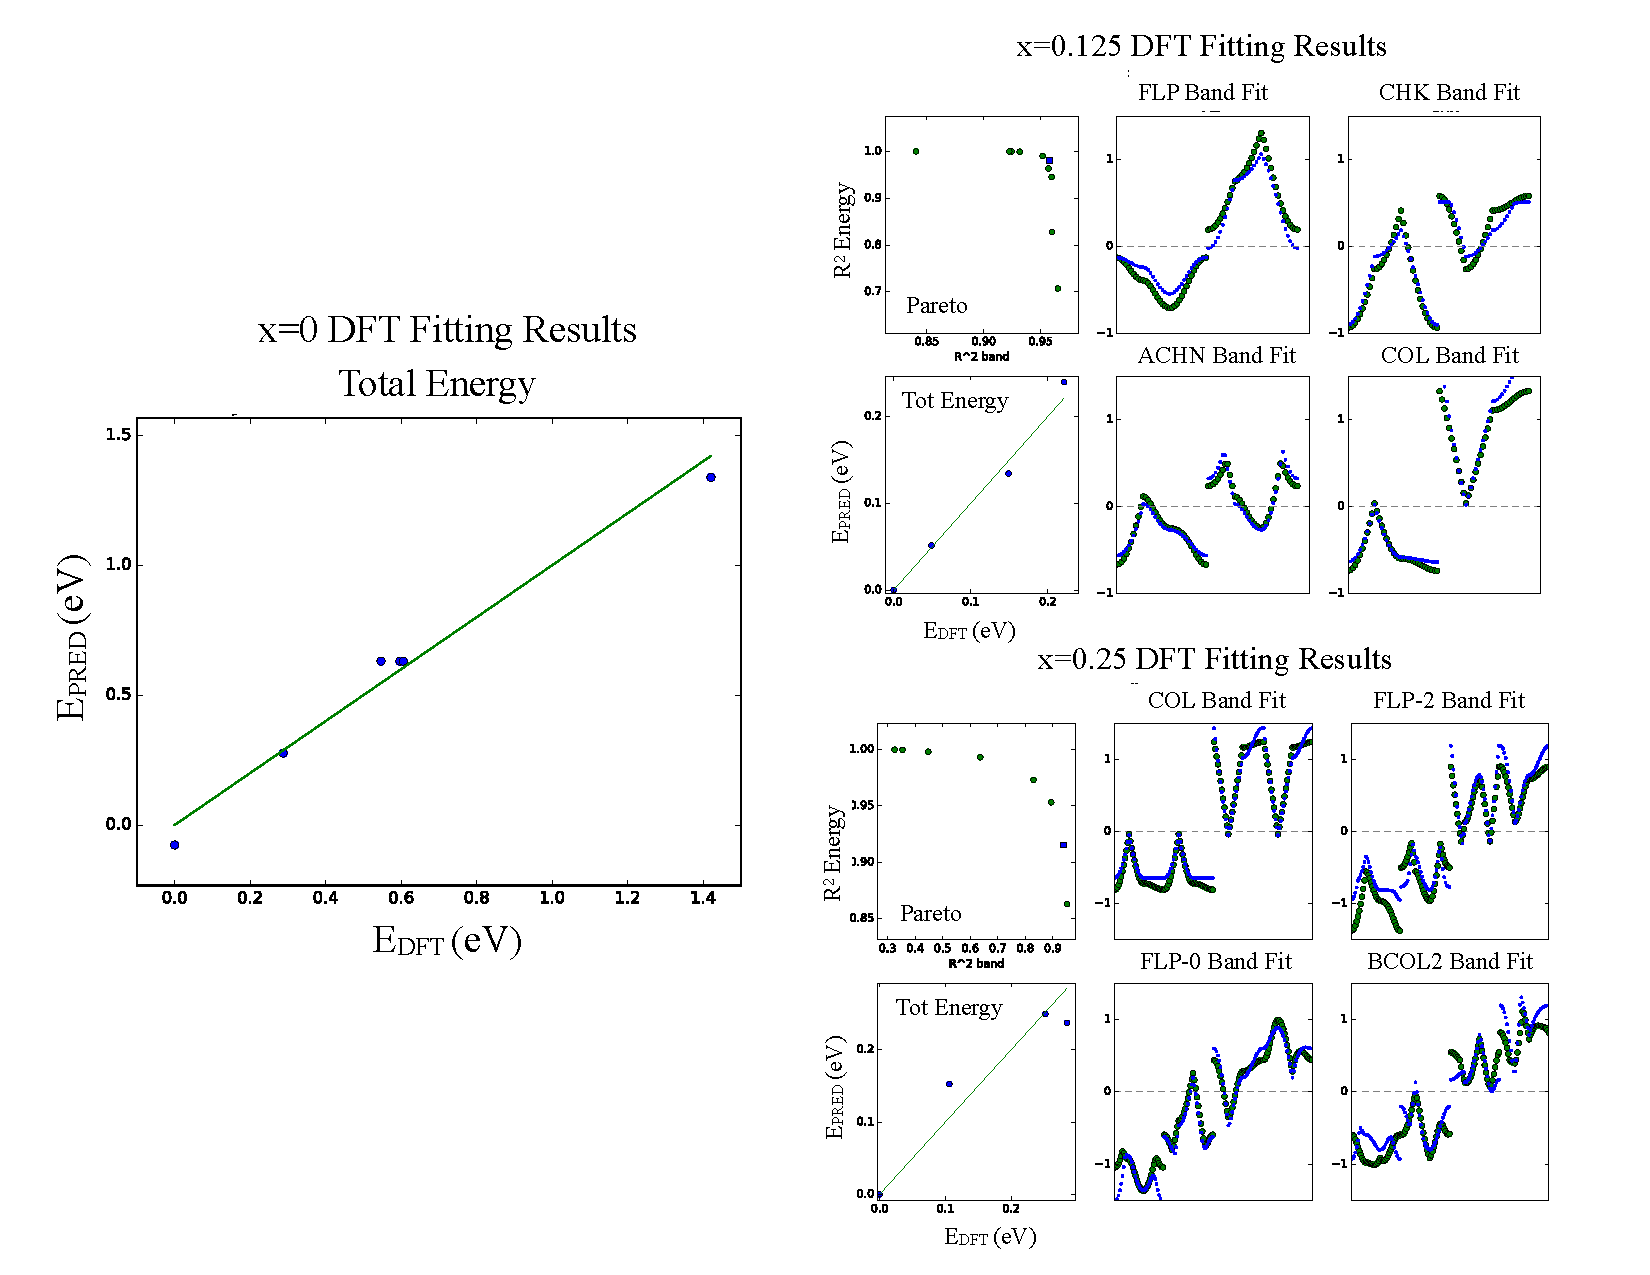
\includegraphics[width=0.9\textwidth]{Figures/R2-pareto.pdf}
\caption{\label{fig4} Results of the \textit{ad hoc} fitting procedure just using the DFT eigenvalues and total energies for three different dopings.}
\end{figure}

\begin{figure}[H]
\centering
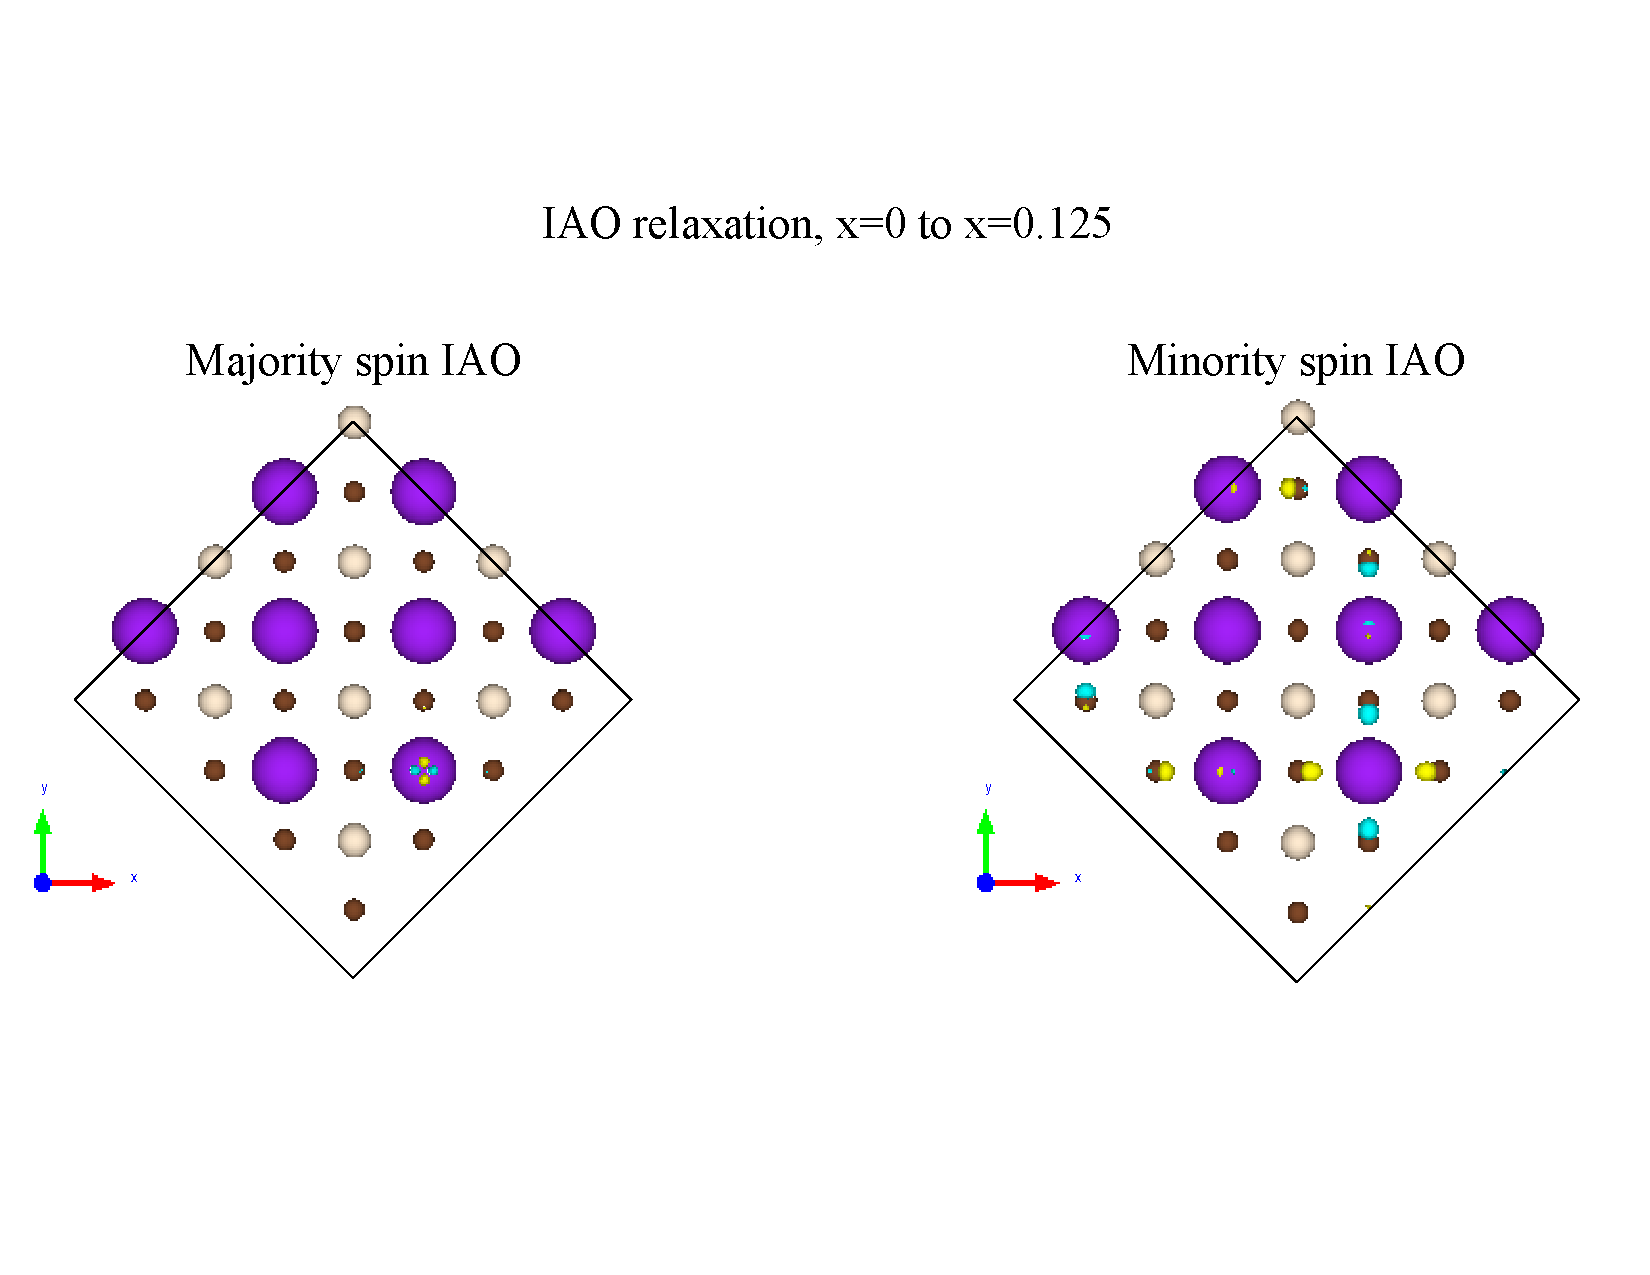
\includegraphics[width=0.9\textwidth]{Figures/R3-iao_basis.pdf}
\caption{\label{fig5} Relaxation of the IAOs for the spin majority and minority channel under doping for the eighth doped flip state. The majority spin IAO can be used as a basis for the fixed spin moments and the minority spin IAO for the itinerant electrons.}
\end{figure}

%\section{References}
%\begin{enumerate}
%\item https://journals.aps.org/rmp/abstract/10.1103/RevModPhys.82.2421
%\item https://journals.aps.org/prl/abstract/10.1103/PhysRevLett.62.2751
%\item https://www.nature.com/articles/375561a0
%\item https://journals.aps.org/prb/abstract/10.1103/PhysRevB.54.7489
%\item https://journals.aps.org/prb/abstract/10.1103/PhysRevB.60.3643
%\item https://www.nature.com/articles/nphys178
%\end{enumerate}
 
\end{document}